\documentclass[10pt]{article}
\usepackage{setspace}
\usepackage{amsmath,amssymb}
\usepackage{amsthm}
\usepackage{fancybox}
\usepackage{algorithm, algpseudocode}
\usepackage{url}



\usepackage{enumitem}
\usepackage{multirow}
\usepackage{color}
\usepackage{graphicx}
\usepackage{setspace}
\usepackage{comment}
\usepackage{bm}

\begingroup
\renewcommand{\section}[2]{}%
%\renewcommand{\chapter}[2]{}% for othe

\newcommand*{\KeepStyleUnderBrace}[1]{%f
  \mathop{%
    \mathchoice
    {\underbrace{\displaystyle#1}}%
    {\underbrace{\textstyle#1}}%
    {\underbrace{\scriptstyle#1}}%
    {\underbrace{\scriptscriptstyle#1}}%
  }\limits
}


\usepackage[margin=0.85in]{geometry}
 
\allowdisplaybreaks[4]
\usepackage{bbm}


\usepackage{amsrefs}
\usepackage{mathtools}
\mathtoolsset{showonlyrefs=true}


\usepackage[utf8]{inputenc}
\usepackage{hyperref}
\hypersetup{
    colorlinks=true,
    citecolor = blue,
    linkcolor=blue,
    filecolor=magenta,           
    urlcolor=cyan,
}

\usepackage[breakable, theorems, skins]{tcolorbox}
\DeclareRobustCommand{\mybox}[2][gray!20]{%
\begin{tcolorbox}[   %% Adjust the following parameters at will.
        breakable,
        left=0pt,
        right=0pt,
        top=0pt,
        bottom=0pt,
        colback=#1,
        colframe=#1,
        width=\dimexpr\textwidth\relax, 
        enlarge left by=0mm,
        boxsep=5pt,
        arc=0pt,outer arc=0pt,
        ]
        #2
\end{tcolorbox}
}


\theoremstyle{plain}
\newtheorem{thm}{Theorem}

\theoremstyle{definition}
\newtheorem{open}[]{Open problems}

 \usepackage[parfill]{parskip}


\input macros.tex

\begin{document}
\begin{center}
\vspace{.2cm}
{\bf \large Tensor Methods and Applications to Biomedical Challenges}\\
\vspace{.1cm}
Miaoyan Wang, Department of Statistics}
\\
\end{center}
\vspace{.2cm}

I work at the intersection of {\bf statistics}, {\bf machine learning}, and {\bf nuroimaging}, with a particular focus on higher-order tensor methods. My research is driven by data analytic problems in {\bf signal processing and data fusion}. These problems often involve large-scale, high-dimensional data, for which novel statistical methods are required. Examples include data from multi-relational social networks and context-specific recommendation systems. {\bf The proposed project is to develop a framework of statistical models, efficient algorithms, and mathematical theory to analyze large-scale tensor data.} Through the development of analytic tools for big tensor data, my research aims at increasing the efficiency in biomedical discoveries. 

{\bf Tensor methods transform data to knowledge}


Tensors are high-dimensional arrays (Figure~\ref{fig:1}a). Recent advances in high-throughput technology have transformed scientific research into data-intensive fields where data are naturally generated in tensor form. Figure~\ref{fig:1}b illustrates an example of tensor data arising from my current collaboration on multi-modal imaging analysis of brain connectivity. The Human Connectome Project provides a huge compendium of tensor data consisting of anatomical and functional connectivities within 1,200 human brains. Multiple imaging measurements are utilized to construct the brain networks, including functional magnetic resonance imaging (fMRI), electroencephalography (EEG), and diffusion tensor imaging (DTI). Understanding key patterns among multimodal networks is crucial to unravel brain functions, thereby broadly facilitating research efforts towards personalized treatment for human diseases. 


\begin{figure}[H]
\begin{center}
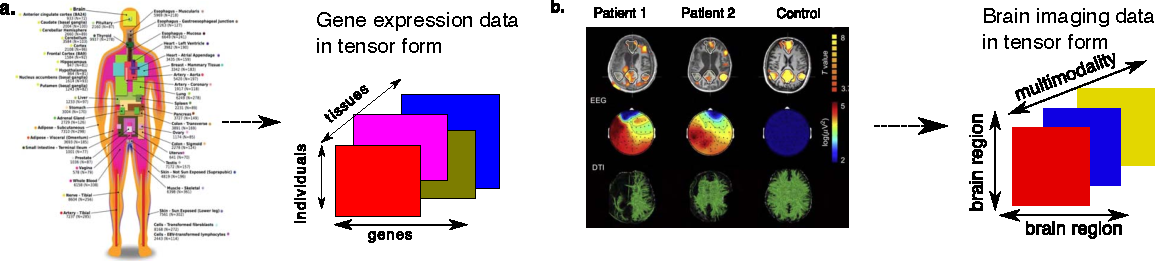
\includegraphics[width=1\textwidth]{example.pdf}
\caption{\small (a) Higher-order tensors are generalizations of matrices. (b) Tensor data from neuroimaging studies. Multiple measurements are used to construct brain connectivities within 1,200 individuals (Bruno et al., 2011).}\label{fig:1}
\end{center}
\end{figure} 
\vspace{-.4cm}

Methods built on tensors provide generalized tools to capture complex data structure that the off-the-shelf methods may fail to exploit. In many data fusion applications, researcher are interested in interpretable low-dimensional structure within the high-dimensional tensor data. The question goes beyond the traditional multivariate analysis; we aim to characterize probabilistic distributions over higher-order ``objects'', where the objects can be images, networks, manifolds, or in general, tensors. Our project targets at developing theory, methodology, and practice for analyzing high-dimensional data. {\bf The resulting prototypes will facilitate automatic detection of hidden salient structure in tensor data, thereby providing solutions to questions that cannot be addressed by classical methods.} 


The proposal focuses on two main directions outlined below. The ultimate goal is to not only bridge data analytics to domain science, but also spark new areas where machine learning theory and scientific discovery can complement each other.

{\bf Project 1: Supervised learning with high-dimensional tensors.} Prediction machine learning problems common arise in daily applications, i.e.,\ identifying segmentations from images, classifying documents into topics, or deciding target customers in recommendation systems. These problems are often formulated as predicting a variable $Y$ from explanatory variables $X$, where the data available is in the form of pairs $\{(X_i, Y_i): i=1,\ldots,n\}$. In contrast to traditional work that focuses on only univariate response, we will develop a general learning framework with tensor observation serving as a response, and features along multiple modes forming the predictor. The proposed model enables the prediction of a high-dimensional tensor $Y\in\mathbb{R}^{d_1\times \cdots \times d_K}$ from possibly multiple predictors $X^{(k)}\in\mathbb{R}^{d_k\times p_k}$, where $k=1,\ldots,K$ indexes the modes of the tensor. The tensor approach boosts the prediction performance by incorporation of multi-way information across the different modes. 


The learning problem is challenging because of the extremely high dimensionality in the tensor parameter space. The PI's previous extensive experience on tensor related work has shown that tensors sought in applications often possess special structures, such as (nearly) low-rankness, sparsity, non-negativity, or orthogonal decomposability. We will leverage the formalisms of \emph{intrinsic dimension} to develop efficient statistical methods for analyzing these high-dimensional datasets. We will further develop adaptive, semi-supervised methods that incorporate practical constraints in insurance applications, such as incomplete observation with missing labels, corrupted distributions, and computation with time and memory constraints. 

\mybox[gray!20]{{\bf Impact and Significance:} 
\begin{itemize}[leftmargin=*]
\item Develop efficient prediction tools for tensor classification, tensor regression, and deep tensor neural network in the presence of domain constraints.
\item Build data-driven prototypes that integrate machine learning into the data-to-decision process. 
\item Improve efficiency in biomedical discovery using powerful multi-modal brain imaging analyses. 
\end{itemize}
}

{\bf Project 2: Unsupervised learning with high-dimensional tensors.} My goal in this direction is to develop unsupervised learning tools, i.e., clustering, denoising, and dimension reduction, for high-dimensional tensors, where the learner has little or no label information during training. This is an area where modeling and validation are notably difficult due to missing information. My group has recently developed an efficient tensor decomposition method to successfully estimate salient blocks in the multi-relational network data. Our clustering algorithm discovers community structure with higher accuracy, while being $11\times$ faster, than the competing methods. We are currently generalizing the methods for integrative analysis of multimodality networks. The work will unlock several ambitious directions that lead to robust decision-making in science, engineering, biomedical applications including health industry.  

\mybox[gray!20]{
{\bf Impact and Significance:} 
\begin{itemize}[leftmargin=*]
\item Develop interactive data exploration and visualization for unsupervised learning tasks such as tensor clustering, density estimation, and dimension reduction. 
\item Design robust tools to analyze tensor data and extract hidden information to aid biomedical decision making. 
\item Address data mining challenges from information gathering to pattern recognition. 
\end{itemize}
 }

{\bf Deliverables and Milestones.}
I am one of the few young faculty members in Statistics. My group consists of three PhD students and two Master/undergraduates, of which three are females (me included) and three are males. I have been actively contributed to several multi-institutional consortiums, in collaboration with researchers in United States, France, and China. This grant will support me to further create a diverse working group. The following table summarizes the planned milestones for my proposal. 
\vspace{-.4cm}
\begin{center}
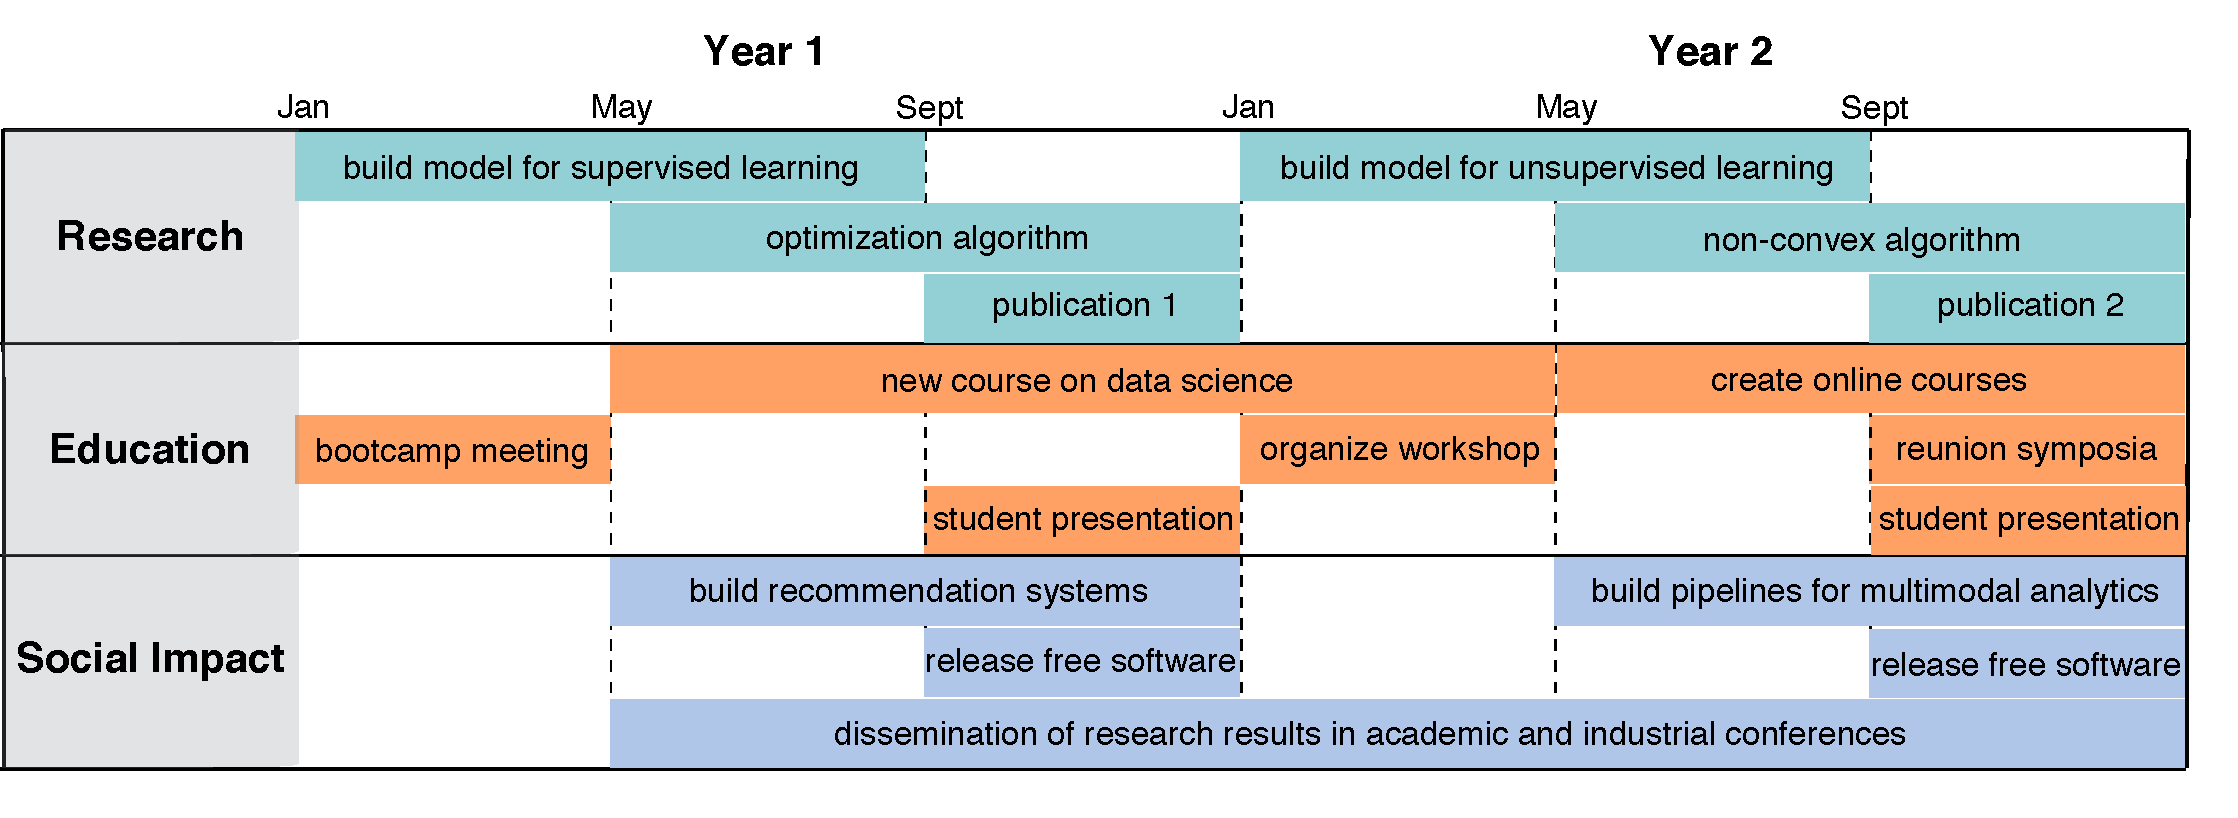
\includegraphics[width=.98\textwidth]{milestone.pdf}
\end{center}
\vspace{-.4cm}
The project will create deliverables in three aspects: {\bf research}, {\bf education}, and {\bf social good}. I plan to devote one year for each of the aforementioned research problems. Regarding teaching, I will create a new course on \emph{data science} in both traditional and online formats. The new course will introduce students to the real word challenges in implementing statistical machine learning approaches to decision making. Open-source software will be released, as the fruit of the research, that facilitates academia, industry, and society to analyze complicated tensor data. The PI will organize a series of workshops on the scientific applications of tensor data analysis, with the aim to encourage interdisciplinary collaborations. 
\end{document}